\documentclass[tikz, border=8pt]{standalone}
\usepackage{tikz}
\usepackage{helvet}
\usetikzlibrary{shapes.geometric, arrows.meta, positioning, fit, backgrounds, shadows}

% --- Color palette ---
\definecolor{colA}{HTML}{D94F3D}  % No training - red
\definecolor{colB}{HTML}{E8A838}  % Moderate - amber
\definecolor{colC}{HTML}{3A7D44}  % Extended - green
\definecolor{colHead}{HTML}{2C3E6B}  % Dark blue headers
\definecolor{colBg}{HTML}{F4F6FB}   % Light panel bg
\definecolor{colArrow}{HTML}{555555}
\definecolor{colBox}{HTML}{DDEAF6}

\begin{document}
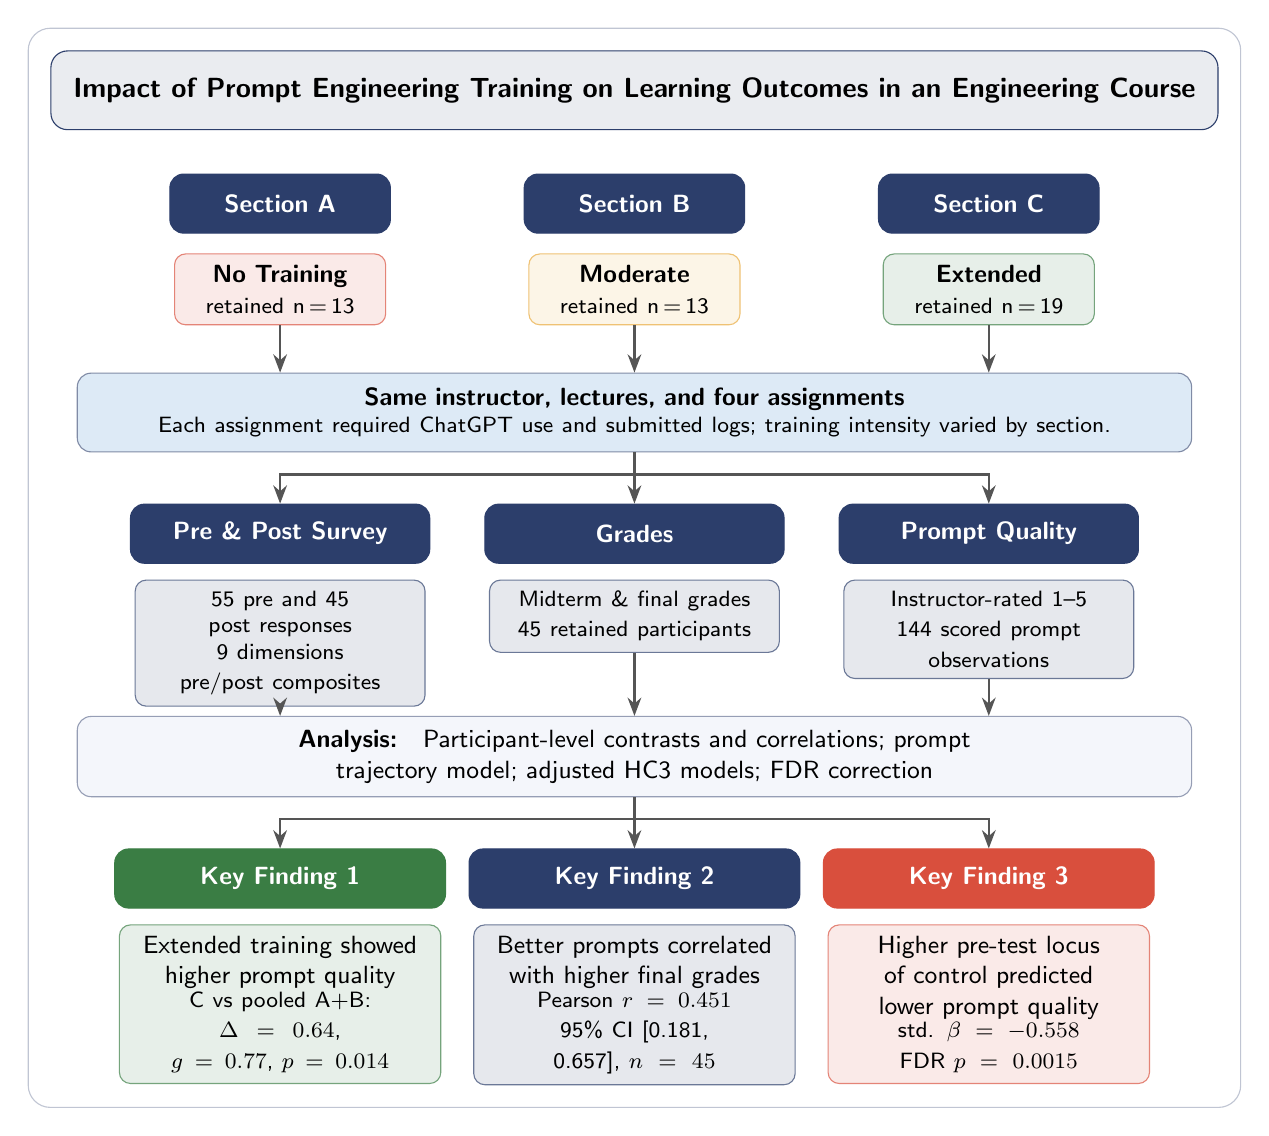
\begin{tikzpicture}[
  font=\sffamily\small,
  >=Stealth,
  every node/.style={align=center},
  box/.style={
    rounded corners=4pt, draw=#1!70, fill=#1!12,
    minimum width=2.6cm, minimum height=0.9cm,
    text width=2.4cm, inner sep=4pt
  },
  headerbox/.style={
    rounded corners=5pt, draw=colHead, fill=colHead,
    text=white, font=\sffamily\bfseries\small,
    minimum width=2.8cm, minimum height=0.75cm,
    inner sep=4pt
  },
  arrow/.style={->, thick, color=colArrow},
  dasharrow/.style={->, thick, dashed, color=colArrow},
]

%% ============================================================
%% ROW 0 - Title strip
%% ============================================================
\node[draw=colHead, fill=colHead!10, rounded corners=6pt,
      text width=14.4cm, minimum height=1.0cm,
      font=\sffamily\bfseries\normalsize, inner sep=6pt]
  (title) at (0,0)
  {Impact of Prompt Engineering Training on Learning Outcomes in an Engineering Course};

%% ============================================================
%% ROW 1 - Three sections / arms
%% ============================================================
\node[headerbox, below=0.55cm of title, xshift=-4.5cm] (secA) {Section A};
\node[headerbox, below=0.55cm of title]                (secB) {Section B};
\node[headerbox, below=0.55cm of title, xshift=+4.5cm] (secC) {Section C};

\node[box=colA, below=0.25cm of secA, text width=2.4cm]
  (trainA) {\textbf{No Training}\\ {\footnotesize retained n\,=\,13}};
\node[box=colB, below=0.25cm of secB, text width=2.4cm]
  (trainB) {\textbf{Moderate}\\ {\footnotesize retained n\,=\,13}};
\node[box=colC, below=0.25cm of secC, text width=2.4cm]
  (trainC) {\textbf{Extended}\\ {\footnotesize retained n\,=\,19}};

%% ============================================================
%% ROW 2 - Shared curriculum (spanning all three)
%% ============================================================
\node[draw=colHead!60, fill=colBox, rounded corners=5pt,
      text width=13.8cm, minimum height=1.0cm, inner sep=5pt,
      below=0.6cm of trainB]
  (curriculum)
  {\textbf{Same instructor, lectures, and four assignments}\\[-1pt]
   {\footnotesize Each assignment required ChatGPT use and submitted logs; training intensity varied by section.}};

%% ============================================================
%% ROW 3 - Data collected
%% ============================================================
\node[headerbox, below=0.65cm of curriculum, xshift=-4.5cm, minimum width=3.8cm]
  (d1h) {Pre \& Post Survey};
\node[headerbox, below=0.65cm of curriculum, minimum width=3.8cm]
  (d2h) {Grades};
\node[headerbox, below=0.65cm of curriculum, xshift=+4.5cm, minimum width=3.8cm]
  (d3h) {Prompt Quality};

\node[box=colHead, below=0.20cm of d1h, text width=3.4cm, minimum width=3.6cm]
  (d1) {{\footnotesize 55 pre and 45 post responses\\9 dimensions\\pre/post composites}};
\node[box=colHead, below=0.20cm of d2h, text width=3.4cm, minimum width=3.6cm]
  (d2) {{\footnotesize Midterm \& final grades\\45 retained participants}};
\node[box=colHead, below=0.20cm of d3h, text width=3.4cm, minimum width=3.6cm]
  (d3) {{\footnotesize Instructor-rated 1--5\\144 scored prompt observations}};

%% ============================================================
%% ROW 4 - Analysis
%% ============================================================
\node[draw=colHead!50, fill=colBg, rounded corners=5pt,
      text width=13.8cm, minimum height=0.85cm, inner sep=5pt,
      below=0.8cm of d2]
  (analysis)
  {\textbf{Analysis:}\quad Participant-level contrasts and correlations; prompt trajectory model; adjusted HC3 models; FDR correction};

%% ============================================================
%% ROW 5 - Key findings (3 boxes)
%% ============================================================
\node[headerbox, below=0.65cm of analysis, xshift=-4.5cm, minimum width=4.2cm,
      fill=colC, draw=colC]
  (f1h) {Key Finding 1};
\node[headerbox, below=0.65cm of analysis, minimum width=4.2cm,
      fill=colHead, draw=colHead]
  (f2h) {Key Finding 2};
\node[headerbox, below=0.65cm of analysis, xshift=+4.5cm, minimum width=4.2cm,
      fill=colA, draw=colA]
  (f3h) {Key Finding 3};

\node[box=colC, below=0.20cm of f1h, text width=3.8cm, minimum width=4.0cm]
  (f1) {Extended training showed higher prompt quality\\[-1pt]
        {\footnotesize C vs pooled A+B:\\$\Delta=0.64$, $g=0.77$, $p=0.014$}};
\node[box=colHead, below=0.20cm of f2h, text width=3.8cm, minimum width=4.0cm]
  (f2) {Better prompts correlated with higher final grades\\[-1pt]
        {\footnotesize Pearson $r=0.451$\\95\% CI [0.181, 0.657], $n=45$}};
\node[box=colA, below=0.20cm of f3h, text width=3.8cm, minimum width=4.0cm]
  (f3) {Higher pre-test locus of control predicted lower prompt quality\\[-1pt]
        {\footnotesize std. $\beta=-0.558$\\FDR $p=0.0015$}};

%% ============================================================
%% ARROWS - training to curriculum to data to analysis to findings
%% ============================================================
\foreach \src in {trainA, trainB, trainC}
  \draw[arrow] (\src.south) -- (\src.south |- curriculum.north);

\draw[arrow] (curriculum.south) -- ++(0,-0.28) -| (d1h.north);
\draw[arrow] (curriculum.south) -- ++(0,-0.28) -| (d2h.north);
\draw[arrow] (curriculum.south) -- ++(0,-0.28) -| (d3h.north);

\foreach \src in {d1, d2, d3}
  \draw[arrow] (\src.south) -- (\src.south |- analysis.north);

\draw[arrow] (analysis.south) -- ++(0,-0.28) -| (f1h.north);
\draw[arrow] (analysis.south) -- ++(0,-0.28) -| (f2h.north);
\draw[arrow] (analysis.south) -- ++(0,-0.28) -| (f3h.north);

%% ============================================================
%% Background panel
%% ============================================================
\begin{scope}[on background layer]
  \node[fill=white, draw=colHead!30, rounded corners=8pt,
        fit=(title)(f1)(f2)(f3), inner sep=8pt] {};
\end{scope}

\end{tikzpicture}
\end{document}
